\documentclass{beamer}

\usepackage{geometry}
\usepackage{graphicx}
%\usepackage{wrapfig}
\usepackage{amsmath}

%\useoutertheme{infolines}
\usetheme{Boadilla}
\usecolortheme{seahorse}
\setbeamertemplate{navigation symbols}{}
\title{High Performance Assembly Programming}
\newcommand{\shorttitle}{64 Bit Intel Assembly Language}
\newcommand{\shortauthor}{\copyright 2011 Ray Seyfarth}
\author{Ray Seyfarth}
\begin{document}


\usefoottemplate{\vbox{
\tinycolouredline{structure!55}%
 {\color{white}{\textbf{\shorttitle}\hfill\textbf{\shortauthor}}}%
}}

\begin{frame}
    \titlepage
\end{frame}

\begin{frame}
\frametitle{Outline}
\tableofcontents
\end{frame}

\section{Optimizations common to C/C++ and assembly}

\begin{frame}
    \frametitle{Use a better algorithm}
    \begin{itemize}
        \item A highly efficient insertion sort is still $O(n^2)$
        \item Using {\tt qsort} from C is generally faster
        \item Using the C++ STL {\tt sort} is faster still
        \item A hash table is $O(1)$ for lookup
        \item In you need an ordered dictionary, perhaps the STL {\tt map} is best
        \item Tuning an $O(n^2)$ algorithm in assembly will not
              convert it to $O(n \lg n)$
    \end{itemize}
\end{frame}

\begin{frame}
    \frametitle{Use C or C++}
    \begin{itemize}
        \item An optimizing compiler will implement nearly all of the
              general optimizations
        \item It will do them tirelessly, missing nearly nothing
        \item Most of a program is not time-critical
        \item Perhaps 10\% of a program is worth optimizing
        \item You must usually find a non-obvious technique to get better
              performance than the compiler
        \item Use the {\tt -S} option to get an assembly listing
        \item Learn the compiler's tricks
        \item Perhaps you can do the compiler's tricks better
    \end{itemize}
\end{frame}

\begin{frame}
    \frametitle{Efficient use of cache}
    \begin{itemize}
        \item The CPU operates at about 3 GHz
        \item Main memory can provide perhaps 7 bytes per machine cycle
        \item Cache is much faster than main memory
        \item Organize your algorithm to work on data in blocks which fit in cache
        \item The plot below shows time versus array size for computing 10 billion
              exclusive or operations
    \end{itemize}
\begin{center}
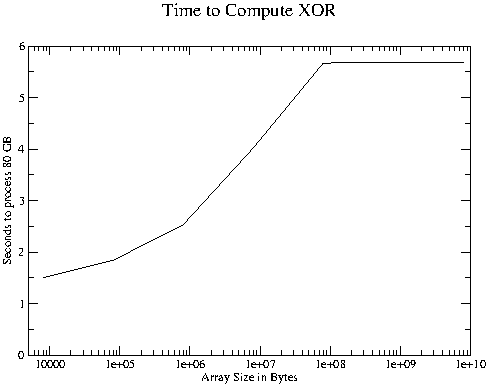
\includegraphics[width=2.4in]{xor.pdf}
\end{center}
\end{frame}

\begin{frame}
    \frametitle{Efficient use of cache(2)}
    \begin{itemize}
        \item The plot below illustrates a dramatic performance gain
              through better use of cache
        \item The task was to compute a $1024\times 1024$ matrix multiplication
        \item The code was written in C using 6 nested loops
        \item The 3 inner-most loops multiplied one block by another
    \end{itemize}
\begin{center}
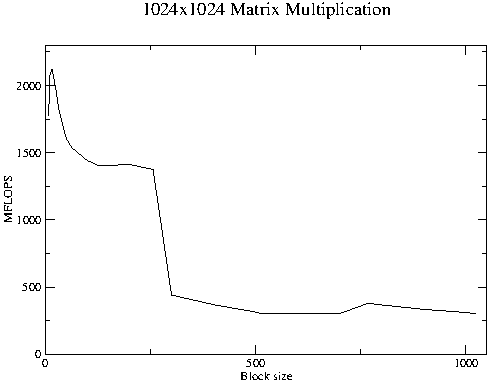
\includegraphics[width=2.4in]{mm.pdf}
\end{center}
\end{frame}

\begin{frame}
    \frametitle{Common sub-expression elimination}
    \begin{itemize}
        \item The compiler will probably do this better than you
        \item You can examine its generated code and perhaps notice
              something you have overlooked
        \item I would bet my money of the compiler with this trick
    \end{itemize}
\end{frame}

\begin{frame}
    \frametitle{Strength reduction}
    \begin{itemize}
        \item This refers to using a simpler mathematical technique
        \item Dividing an integer by 8 could be a shift right 3 bits
        \item Getting a remainder after division by 1024, can be done using {\tt and}
        \item Rather than using {\tt pow(x,3)} use {\tt x*x*x}
        \item Computer $x^4$ by computing $x^2$ and then squaring that
        \item Avoid division by a floating point number $x$, but computing $1/x$ and
              use multiplication instead
        \item Again the compiler will do this tirelessly
    \end{itemize}
\end{frame}

\section{Optimizations the compiler can do in C, but you only in assembly}

\begin{frame}
    \frametitle{Use registers efficiently}
    \begin{itemize}
        \item The compiler will do this automatically
        \item Place commonly-used values in registers
        \item If you unroll a loop, use different registers
              to allow parallel execution of parts of your computation
    \end{itemize}

\end{frame}

\begin{frame}
    \frametitle{Use fewer branches}
    \begin{itemize}
        \item Branches interrupt the instruction pipeline
        \item The compiler will frequently re-order blocks of code to
              reduce branches
        \item Study the compiler's generated code
        \item Use conditional moves for simple computations
    \end{itemize}

\end{frame}

\begin{frame}[fragile]
    \frametitle{Convert loops to branch at the bottom}
    \begin{itemize}
        \item The compiler generally does this to reduce the number of instructions
              in a loop and, especially, the number of branches
        \item Here is a C {\tt for} loop
    \end{itemize}
\begin{verbatim}
        for ( i = 0; i < n; i++ ) {
            x[i] = a[i] + b[i];
        }
\end{verbatim}

    \begin{itemize}
        \item By adding an if at the start you can loop with a branch at the bottom
        \item Don't do this in C.  The compiler will handle this.
    \end{itemize}
\begin{verbatim}
        if ( n > 0 ) {
            i = 0;
            do {
                x[i] = a[i] + b[i];
                i++;
            } while ( i < n );
        }
\end{verbatim}
\end{frame}


\begin{frame}
    \frametitle{Unroll loops}
    \begin{itemize}
        \item Use {\tt -funroll-all-loops} to have {\tt gcc} unroll loops
        \item Unrolling means repeated occurrences of the loop body with
              multiple parts of the data being processed
        \item Try to make each unrolling use different registers to
              reduce instruction dependence
        \item This frees up the CPU to do out-of-order execution
        \item It can do more pipelining and more parallel execution
    \end{itemize}
\end{frame}

\begin{frame}[fragile]
    \frametitle{Assembly code adding numbers in an array, unrolled}
    \begin{itemize}
        \item The addition is done as 4 sub-sums which are added later
        \item The four unrolled parts accumulate into 4 different registers
    \end{itemize}
\begin{verbatim}
.add_words:
        add     rax, [rdi]
        add     rbx, [rdi+8]
        add     rcx, [rdi+16]
        add     rdx, [rdi+16]
        add     rdi, 32
        sub     rsi, 4
        jg      .add_words
        add     rcx, rdx
        add     rax, rbx
        add     rax, rcx
\end{verbatim}
\end{frame}

\begin{frame}[fragile]
    \frametitle{Merge loops}
    \begin{itemize}
        \item If 2 loops have some loop limits, consider merging the bodies
        \item There will be less loop overhead
        \item The following 2 loops can be profitably merged
    \end{itemize}
\begin{verbatim}
        for ( i = 0; i < 1000; i++ ) a[i] = b[i] + c[i];
        for ( j = 0; j < 1000; j++ ) d[j] = b[j] - c[j];
\end{verbatim}
    \begin{itemize}
        \item After merging values for {\tt b[i]} and {\tt c[i]} can be used twice
    \end{itemize}

\begin{verbatim}
        for ( i = 0; i < 1000; i++ ) {
            a[i] = b[i] + c[i];
            d[i] = b[i] - c[i];
        }
\end{verbatim}
\end{frame}

\begin{frame}
    \frametitle{Split loops}
    \begin{itemize}
        \item Didn't I just suggest merging loops?
        \item Sometimes the data is unrelated and merging doesn't help
        \item Perhaps splitting uses cache better
        \item Test your code
    \end{itemize}
\end{frame}

\begin{frame}[fragile]
    \frametitle{Interchange loops}
\begin{verbatim}
        for ( j = 0; j < n; j++ ) {
            for ( i = 0; i < n; i++ ) {
                x[i][j] = 0;
            }
        }
\end{verbatim}
    \begin{itemize}
        \item The previous loop steps through the {\tt x} array in large increments
        \item The loop below steps through the array one element after the other
        \item Cache fetches are better used
    \end{itemize}
\begin{verbatim}
        for ( i = 0; i < n; i++ ) {
            for ( j = 0; j < n; j++ ) {
                x[i][j] = 0;
            }
        }
\end{verbatim}
\end{frame}

\begin{frame}
    \frametitle{Move loop-invariant code outside the loop}
    \begin{itemize}
        \item You can do this in C, but the compiler will do it for you
        \item The assembler does not move loop-invariant code
        \item Again, study the generated code
    \end{itemize}
\end{frame}

\begin{frame}
    \frametitle{Remove recursion}
    \begin{itemize}
        \item Eliminating tail-recursion is generally useful
        \item If you have to simulate a ``stack'' like recursion gives you,
              recursion will probably be faster
    \end{itemize}
\end{frame}


\begin{frame}
    \frametitle{Eliminate stack frames}
    \begin{itemize}
        \item Use {\tt -fomit-frame-pointers} with {\tt gcc}
        \item Use this for debugged code
        \item Using the {\tt rbp} register is optional
        \item Leaf functions don't even need to worry about stack alignment
        \item Unless you are using some local data requiring 16 byte alignment
    \end{itemize}
\end{frame}

\begin{frame}
    \frametitle{Inline functions}
    \begin{itemize}
        \item The compiler can do this painlessly
        \item In assembly you will make your code less readable
        \item Explore using macros
    \end{itemize}
\end{frame}

\section{For assembly only}

\begin{frame}[fragile]
    \frametitle{Reduce dependencies to allow super-scalar execution}
    \begin{itemize}
        \item Use different registers to try to reduce dependencies
        \item The CPU has multiple computational units in 1 core
        \item You can benefit from out-of-order execution
        \item You can get more out of pipelines
        \item You can keep more computational units busy
    \end{itemize}
\end{frame}

\begin{frame}
    \frametitle{Use specialized instructions}
    \begin{itemize}
        \item The compiler will have a harder time doing this than you
        \item There are SIMD integer instructions
        \item There are also SIMD floating point instructions
        \item The AVX instructions are a new feature which allow twice as
              many floating point values in the SIMD registers
    \end{itemize}
\end{frame}

\end{document}
